\documentclass[twoside,10pt]{article}
\usepackage{amsmath,amsfonts,amsthm,fullpage,amssymb}
%\usepackage{mymath}
\usepackage{algorithm,amsmath,amssymb}
\usepackage{algorithmic}
\usepackage{graphicx, color}
\usepackage{url}


\begin{document}


\title{ISYE 6740 Homework 6\\ 
Fall 2020\\
\small Total 100 points.}
\date{}
\maketitle



%As usual, please submit a report with sufficient explanation of your answers to each the questions, together with your code, in a zip folder.

%----------------------------------------------------------------------------------



\begin{enumerate}


\item  {\bf AdaBoost.} (30 points)

Consider the following dataset, plotting in the following figure. The first two coordinates represent the value of two features, and the last coordinate is the binary label of the data.
\begin{equation*}
\begin{split}
&X_1 = (-1, 0, +1), X_2 = (-0.5, 0.5, +1), X_3 = (0, 1, -1), X_4 = (0.5, 1, -1), \\
&X_5 = (1, 0, +1), X_6 = (1, -1, +1), X_7 = (0, -1, -1), X_8 = (0, 0, -1).
\end{split}
\end{equation*}

In this problem, you will run through $T = 3$ iterations of AdaBoost with decision stumps (as explained in the lecture) as weak learners.

\begin{enumerate}
\item (15 points) For each iteration $t = 1, 2, 3$, compute $\epsilon_t$, $\alpha_t$, $Z_t$, $D_t$ by hand (i.e., show the calculation steps) and draw the decision stumps on the figure (you can draw this by hand). 

\item (15 points) What is the training error of this AdaBoost? Give a short explanation for why AdaBoost outperforms a single decision stump.

\end{enumerate}


\vspace{-.2in}
\begin{figure}[h!]
\begin{center}
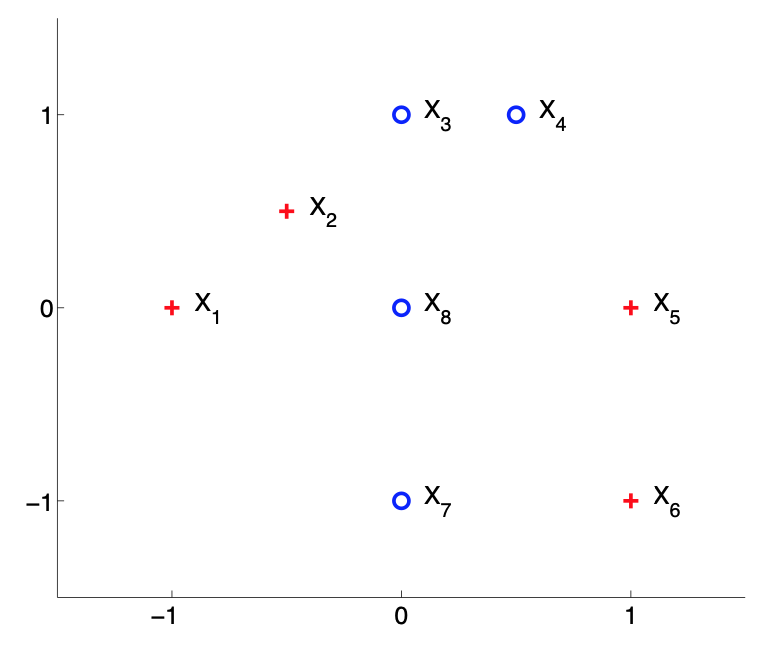
\includegraphics[width =.4 \textwidth]{hw}
\end{center}
%\caption{ A small dataset, for binary classification with AdaBoost.}
\end{figure}
\vspace{-.3in}

\begin{table}
\begin{center}
\caption{Values of AdaBoost parameters at each timestep.}
\vspace{0.1in}
\begin{tabular}{|c|c|c|c|c|c|c|c|c|c|c|c|}\hline
t & $\epsilon_t$ & $\alpha_t$ & $Z_t$ & $D_t(1)$ & $D_t(2)$ & $D_t(3)$ & $D_t(4)$ & $D_t(5)$ & $D_t(6)$ & $D_t(7)$ & $D_t(8)$ \\\hline
1 & & & & & & & & & & & \\
2 & & & & & & & & & & &\\
3 & & & & & & & & & & & \\\hline
\end{tabular}
\end{center}
\end{table}


\clearpage 

\item{\bf Linear regression: bias-variance tradeoff, CV, and variable selection} (30 points)


Consider a dataset with $n$ data points $(x^i, y^i)$, $x^i \in \mathbb R^n$, following from the following linear model:
\[
y^i =  {\beta^*}^T x^i + \epsilon^i, \quad i = 1, \ldots, m,
\]
where $\epsilon^i$ are i.i.d. Gaussian noise with \textcolor{red}{zero mean and variance $\sigma^2$}, and $\beta^*$ is the true parameter. Consider the ridge regression as follows:
\begin{equation} \label{1}
\hat \beta(\lambda) 
= \arg\min_{\beta}
\left\{
\frac 1 m \sum_{i=1}^m (y^i - {\beta}^T x^i)^2 + \lambda \|\beta\|_2^2
\right\},
\end{equation}
where $\lambda \geq 0$ is the regularized parameter. 
\begin{enumerate}
\item (5 points) Find the closed form solution for $\hat \beta(\lambda)$ and its distribution conditioning on $\{x^i\}$ (i.e., treat them as fixed).
\item (5 points) Calculate the bias  $\mathbb E[x^T {\hat \beta}(\lambda)] - x^T {\beta^*}$ as a function of $\lambda$ and some fixed test point $x$.
\item (5 points) Calculate the variance term $\mathbb E\left[\left(x^T {\hat \beta}(\lambda) - \mathbb E[x^T {\hat \beta}(\lambda)] \right)^2\right]$ as a function of $\lambda$.
\item (5 points) Use the results from parts (b) and (c) and the bias-variance decomposition to analyze the impact of $\lambda$ in the \textcolor{red}{mean} squared error. Specifically, which term dominates when $\lambda$ is small, and large, respectively?
\item (5 points) Now suppose we have $m= 100$ samples. Write a pseudo-code to explain how to use cross validation to find the optimal $\lambda$.
\item (5 points) Explain if we would like to perform variable selection, how should we \textcolor{red}{change} the regularization term in Equation (\ref{1}) to achieve this goal. 
\end{enumerate}



\clearpage

\item {\bf Random forest and one-class SVM for email spam classifier} (40 points)

Your task for this question is to build a spam classifier using the UCR email spam dataset \url{https://archive.ics.uci.edu/ml/datasets/Spambase} came from the postmaster and individuals who had filed spam. Please download the data from that website. The collection of non-spam emails came from filed work and personal emails, and hence the word \textsf{'george'} and the area code \textsf{'650'} are indicators of non-spam. These are useful when constructing a personalized spam filter. You are free to choose any package for this homework. Note: there may be some missing values. You can just fill in zero.

\begin{enumerate}

\item (10 points) Build a CART model and visualize the fitted classification tree.

\item (15 points) Now also build a random forest model. Partition the data to use the first 80\% for training and the remaining 20\% for testing. Compare and report the test error for your classification tree and random forest models on testing data. Plot the curve of test error (total misclassification error rate) versus the number of trees for the random forest, and plot the test error for the CART model (which should be a constant with respect to the number of trees). 

\item (15 points) Now we will use a one-class SVM approach for spam filtering. Partition the data to use the first 80\% for training and the remaining 20\% for testing. Extract all {\it non-spam} emails from the training block (80\% of data you have selected) to build the one-class kernel SVM using RBF kernel (you can turn the kernel bandwidth to achieve good performance). Then apply it on the 20\% of data reserved for testing (thus this is a novelty detection situation), and report the total misclassification error rate on these testing data. 

\end{enumerate}


\end{enumerate}





\end{document}
